\tikzset{every picture/.style={line width=0.75pt}} %set default line width to 0.75pt        

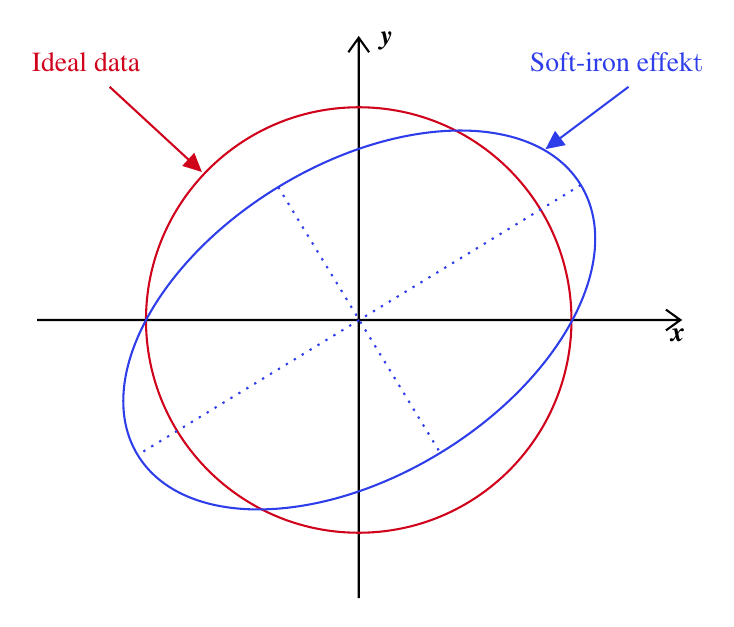
\begin{tikzpicture}[x=0.75pt,y=0.75pt,yscale=-1,xscale=1]
%uncomment if require: \path (0,483); %set diagram left start at 0, and has height of 483

%Shape: Axis 2D [id:dp4165422169263022] 
\draw  (5,236.01) -- (315,236.01)(160,100) -- (160,370) (308,231.01) -- (315,236.01) -- (308,241.01) (155,107) -- (160,100) -- (165,107)  ;
%Shape: Circle [id:dp2065279178112993] 
\draw  [color={rgb, 255:red, 208; green, 2; blue, 27 }  ,draw opacity=1 ] (57.5,236.01) .. controls (57.5,179.4) and (103.39,133.51) .. (160,133.51) .. controls (216.61,133.51) and (262.5,179.4) .. (262.5,236.01) .. controls (262.5,292.62) and (216.61,338.51) .. (160,338.51) .. controls (103.39,338.51) and (57.5,292.62) .. (57.5,236.01) -- cycle ;
%Straight Lines [id:da8202785153086127] 
\draw [color={rgb, 255:red, 208; green, 2; blue, 27 }  ,draw opacity=1 ]   (40,123.67) -- (82.22,162.64) ;
\draw [shift={(84.43,164.67)}, rotate = 222.7] [fill={rgb, 255:red, 208; green, 2; blue, 27 }  ,fill opacity=1 ][line width=0.08]  [draw opacity=0] (8.93,-4.29) -- (0,0) -- (8.93,4.29) -- cycle    ;
%Straight Lines [id:da5890253767345137] 
\draw [color={rgb, 255:red, 46; green, 61; blue, 234 }  ,draw opacity=1 ]   (290,123.67) -- (252.4,151.87) ;
\draw [shift={(250,153.67)}, rotate = 323.13] [fill={rgb, 255:red, 46; green, 61; blue, 234 }  ,fill opacity=1 ][line width=0.08]  [draw opacity=0] (8.93,-4.29) -- (0,0) -- (8.93,4.29) -- cycle    ;
%Shape: Ellipse [id:dp9071994211982046] 
\draw  [color={rgb, 255:red, 46; green, 61; blue, 234 }  ,draw opacity=1 ] (121.23,171.95) .. controls (180.19,136.03) and (245.45,135.59) .. (267,170.97) .. controls (288.55,206.34) and (258.23,264.13) .. (199.27,300.05) .. controls (140.31,335.97) and (75.05,336.41) .. (53.5,301.03) .. controls (31.95,265.66) and (62.27,207.87) .. (121.23,171.95) -- cycle ;
%Straight Lines [id:da4705885477675882] 
\draw [color={rgb, 255:red, 46; green, 61; blue, 234 }  ,draw opacity=1 ] [dash pattern={on 0.84pt off 2.51pt}]  (121.23,171.95) -- (199.27,300.05) ;
%Straight Lines [id:da7090313610480719] 
\draw [color={rgb, 255:red, 46; green, 61; blue, 234 }  ,draw opacity=1 ] [dash pattern={on 0.84pt off 2.51pt}]  (267,170.97) -- (53.5,301.03) ;

% Text Node
\draw (1,105.67) node [anchor=north west][inner sep=0.75pt]  [color={rgb, 255:red, 208; green, 2; blue, 27 }  ,opacity=1 ] [align=left] {{\fontfamily{ptm}\selectfont Ideal data}};
% Text Node
\draw (241,105.67) node [anchor=north west][inner sep=0.75pt]  [color={rgb, 255:red, 46; green, 61; blue, 234 }  ,opacity=1 ] [align=left] {{\fontfamily{ptm}\selectfont Soft-iron effek}t};
% Text Node
\draw (169,95.67) node [anchor=north west][inner sep=0.75pt]   [align=left] {\textit{{\fontfamily{ptm}\selectfont \textbf{y}}}};
% Text Node
\draw (309,238.67) node [anchor=north west][inner sep=0.75pt]   [align=left] {\textit{{\fontfamily{ptm}\selectfont \textbf{x}}}};


\end{tikzpicture}
